\begin{figure}[h!]
    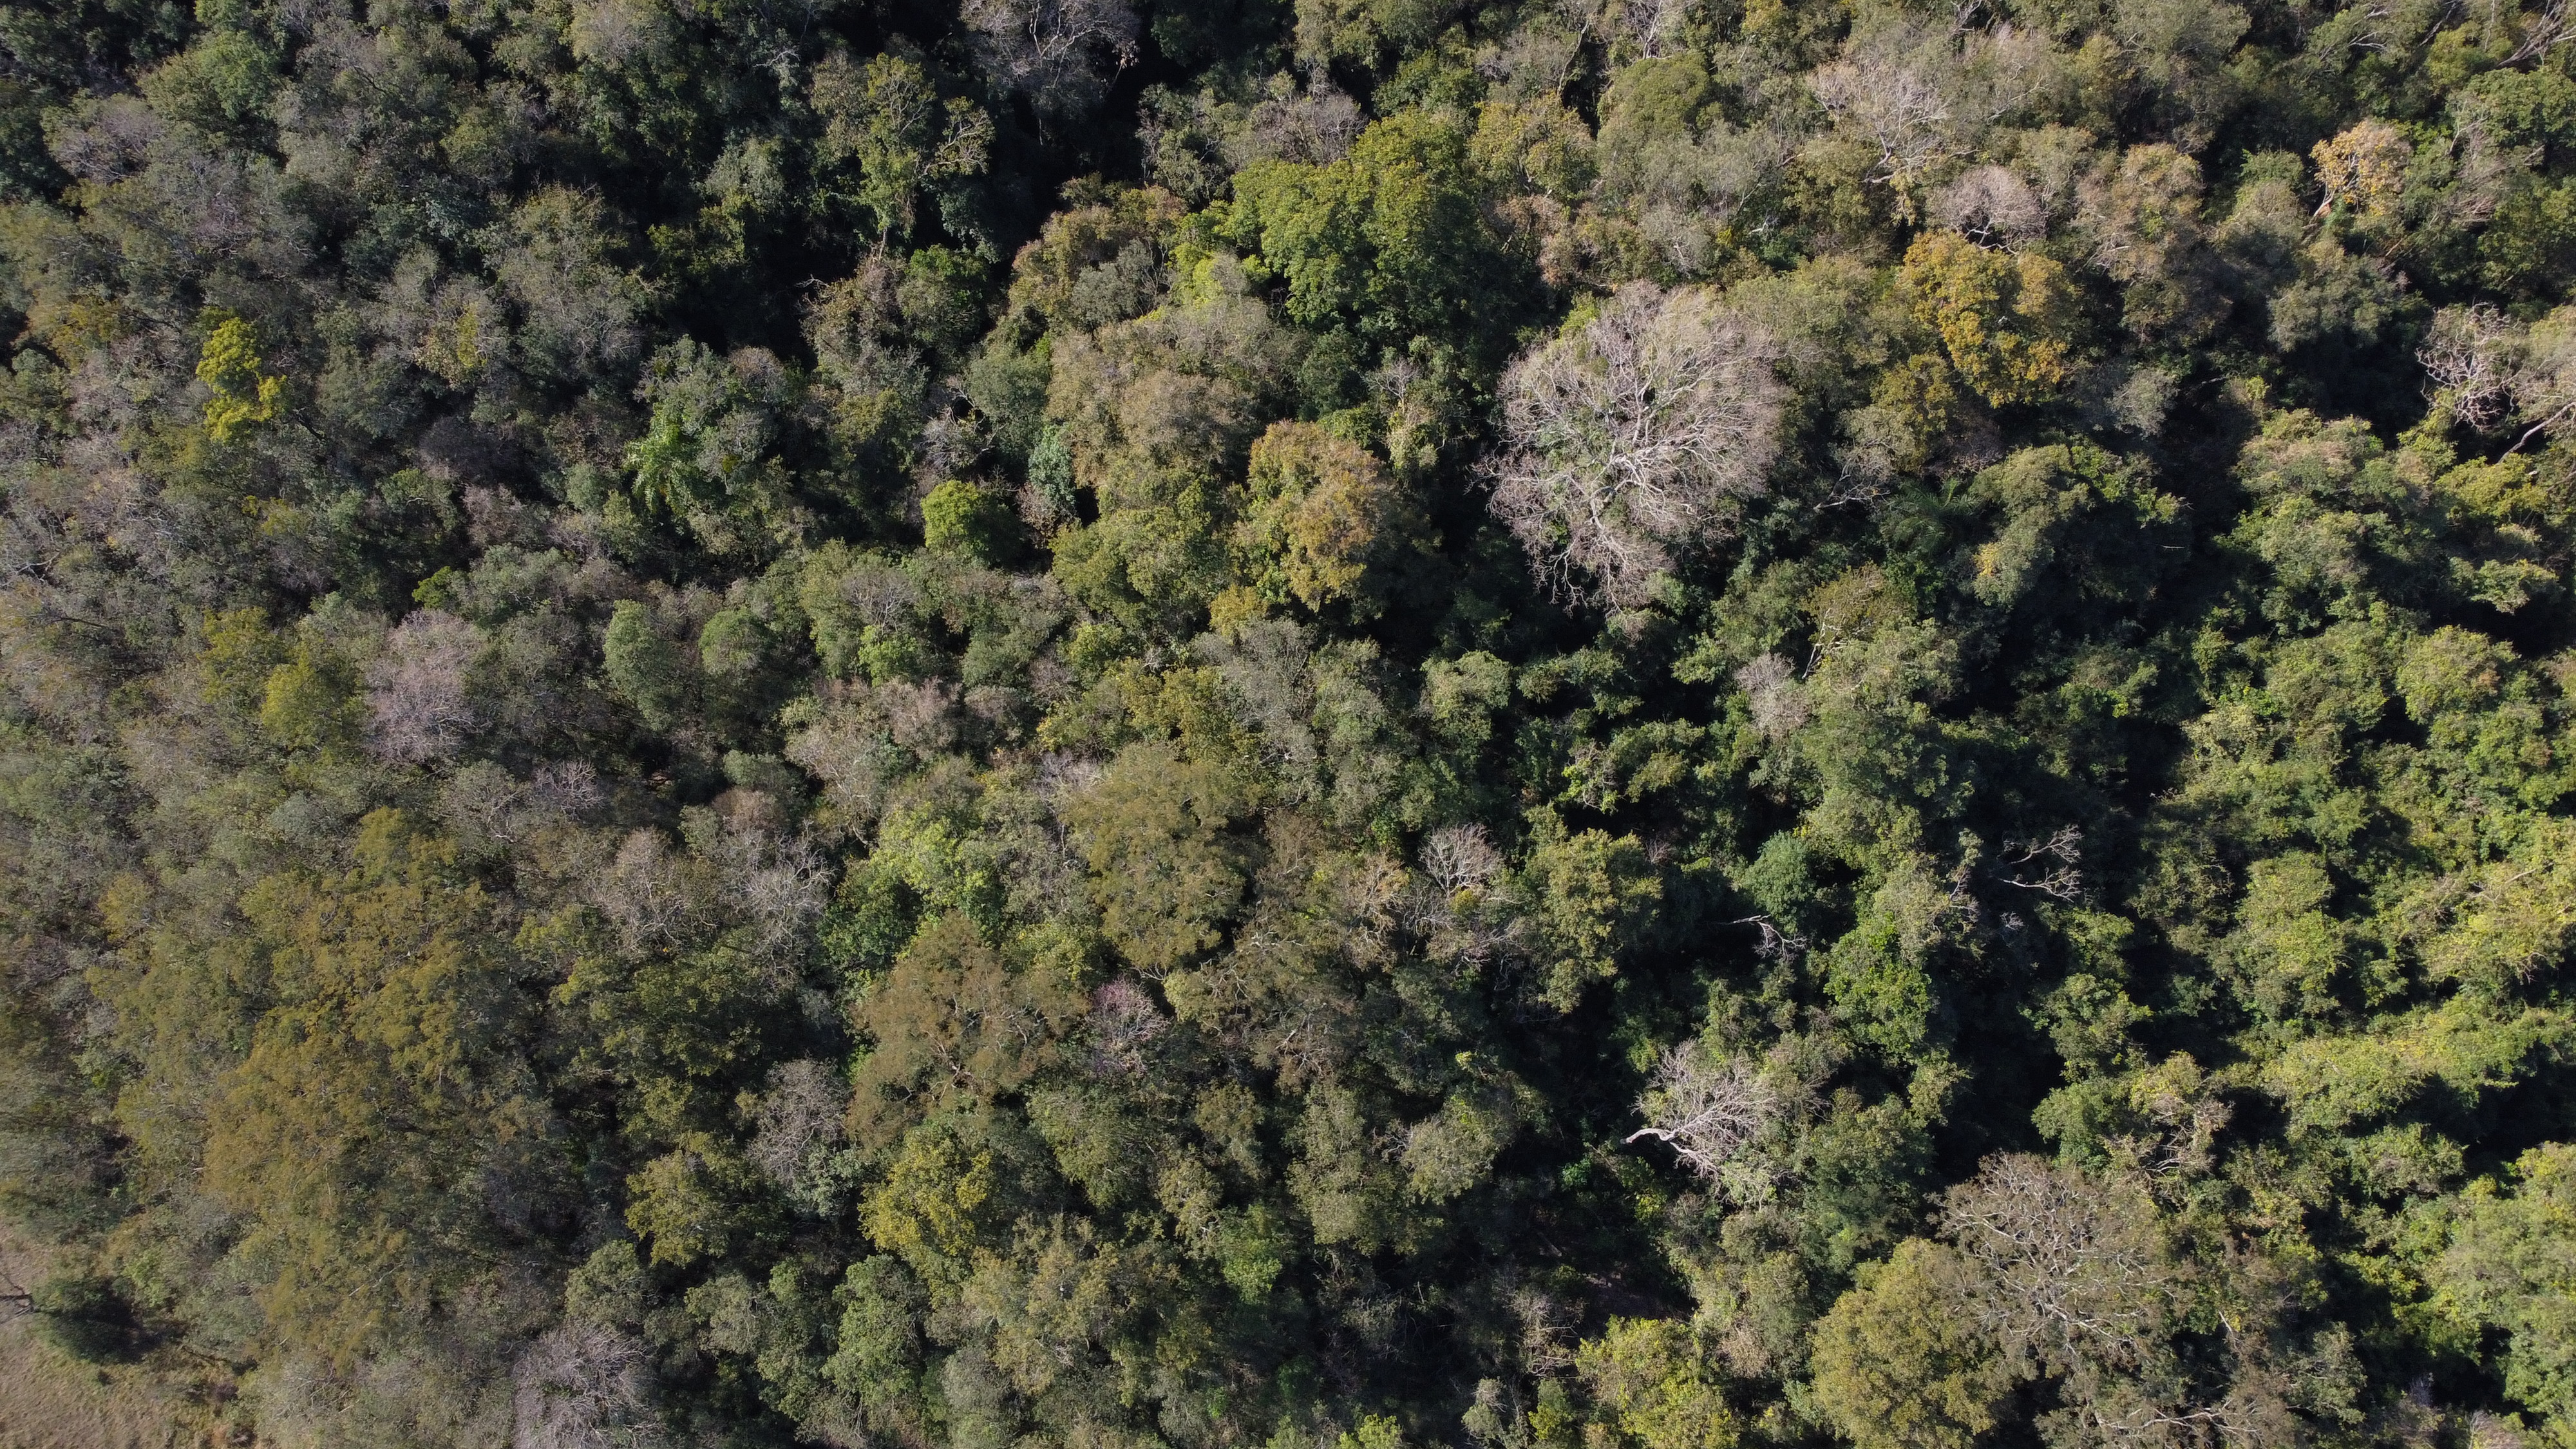
\includegraphics[width=\textwidth]{Imagenes/Homomorfico/DJI_0240.JPG}
     \hfill
     \caption{Imagen aérea (VANT) de reserva provincial Cañadón de Profundidad. Resolución de imagen de N x M píxeles, resolución espacial de X m por píxel.}
    \label{Cañadon_homo}
\end{figure}

\begin{figure}[h!]
    \includegraphics[width=\textwidth]{Imagenes/Homomorfico/DJI_240_bin.png}
     \hfill
     \caption{Máscara binaria obtenida a partir de la imagen de la figura \ref{Cañadon_homo} con umbral de 0,45.}
    \label{mascaraCañadon}
\end{figure}

\begin{figure}[h!]
    \includegraphics[width=\textwidth]{Imagenes/Homomorfico/DJI_240_sel.png}
     \hfill
     \caption{Sombras seleccionadas por el algoritmo a partir de la imagen de la figura \ref{mascaraCañadon}.}
    \label{seleccionadaDJI240}
\end{figure}

\begin{figure}[h!]
    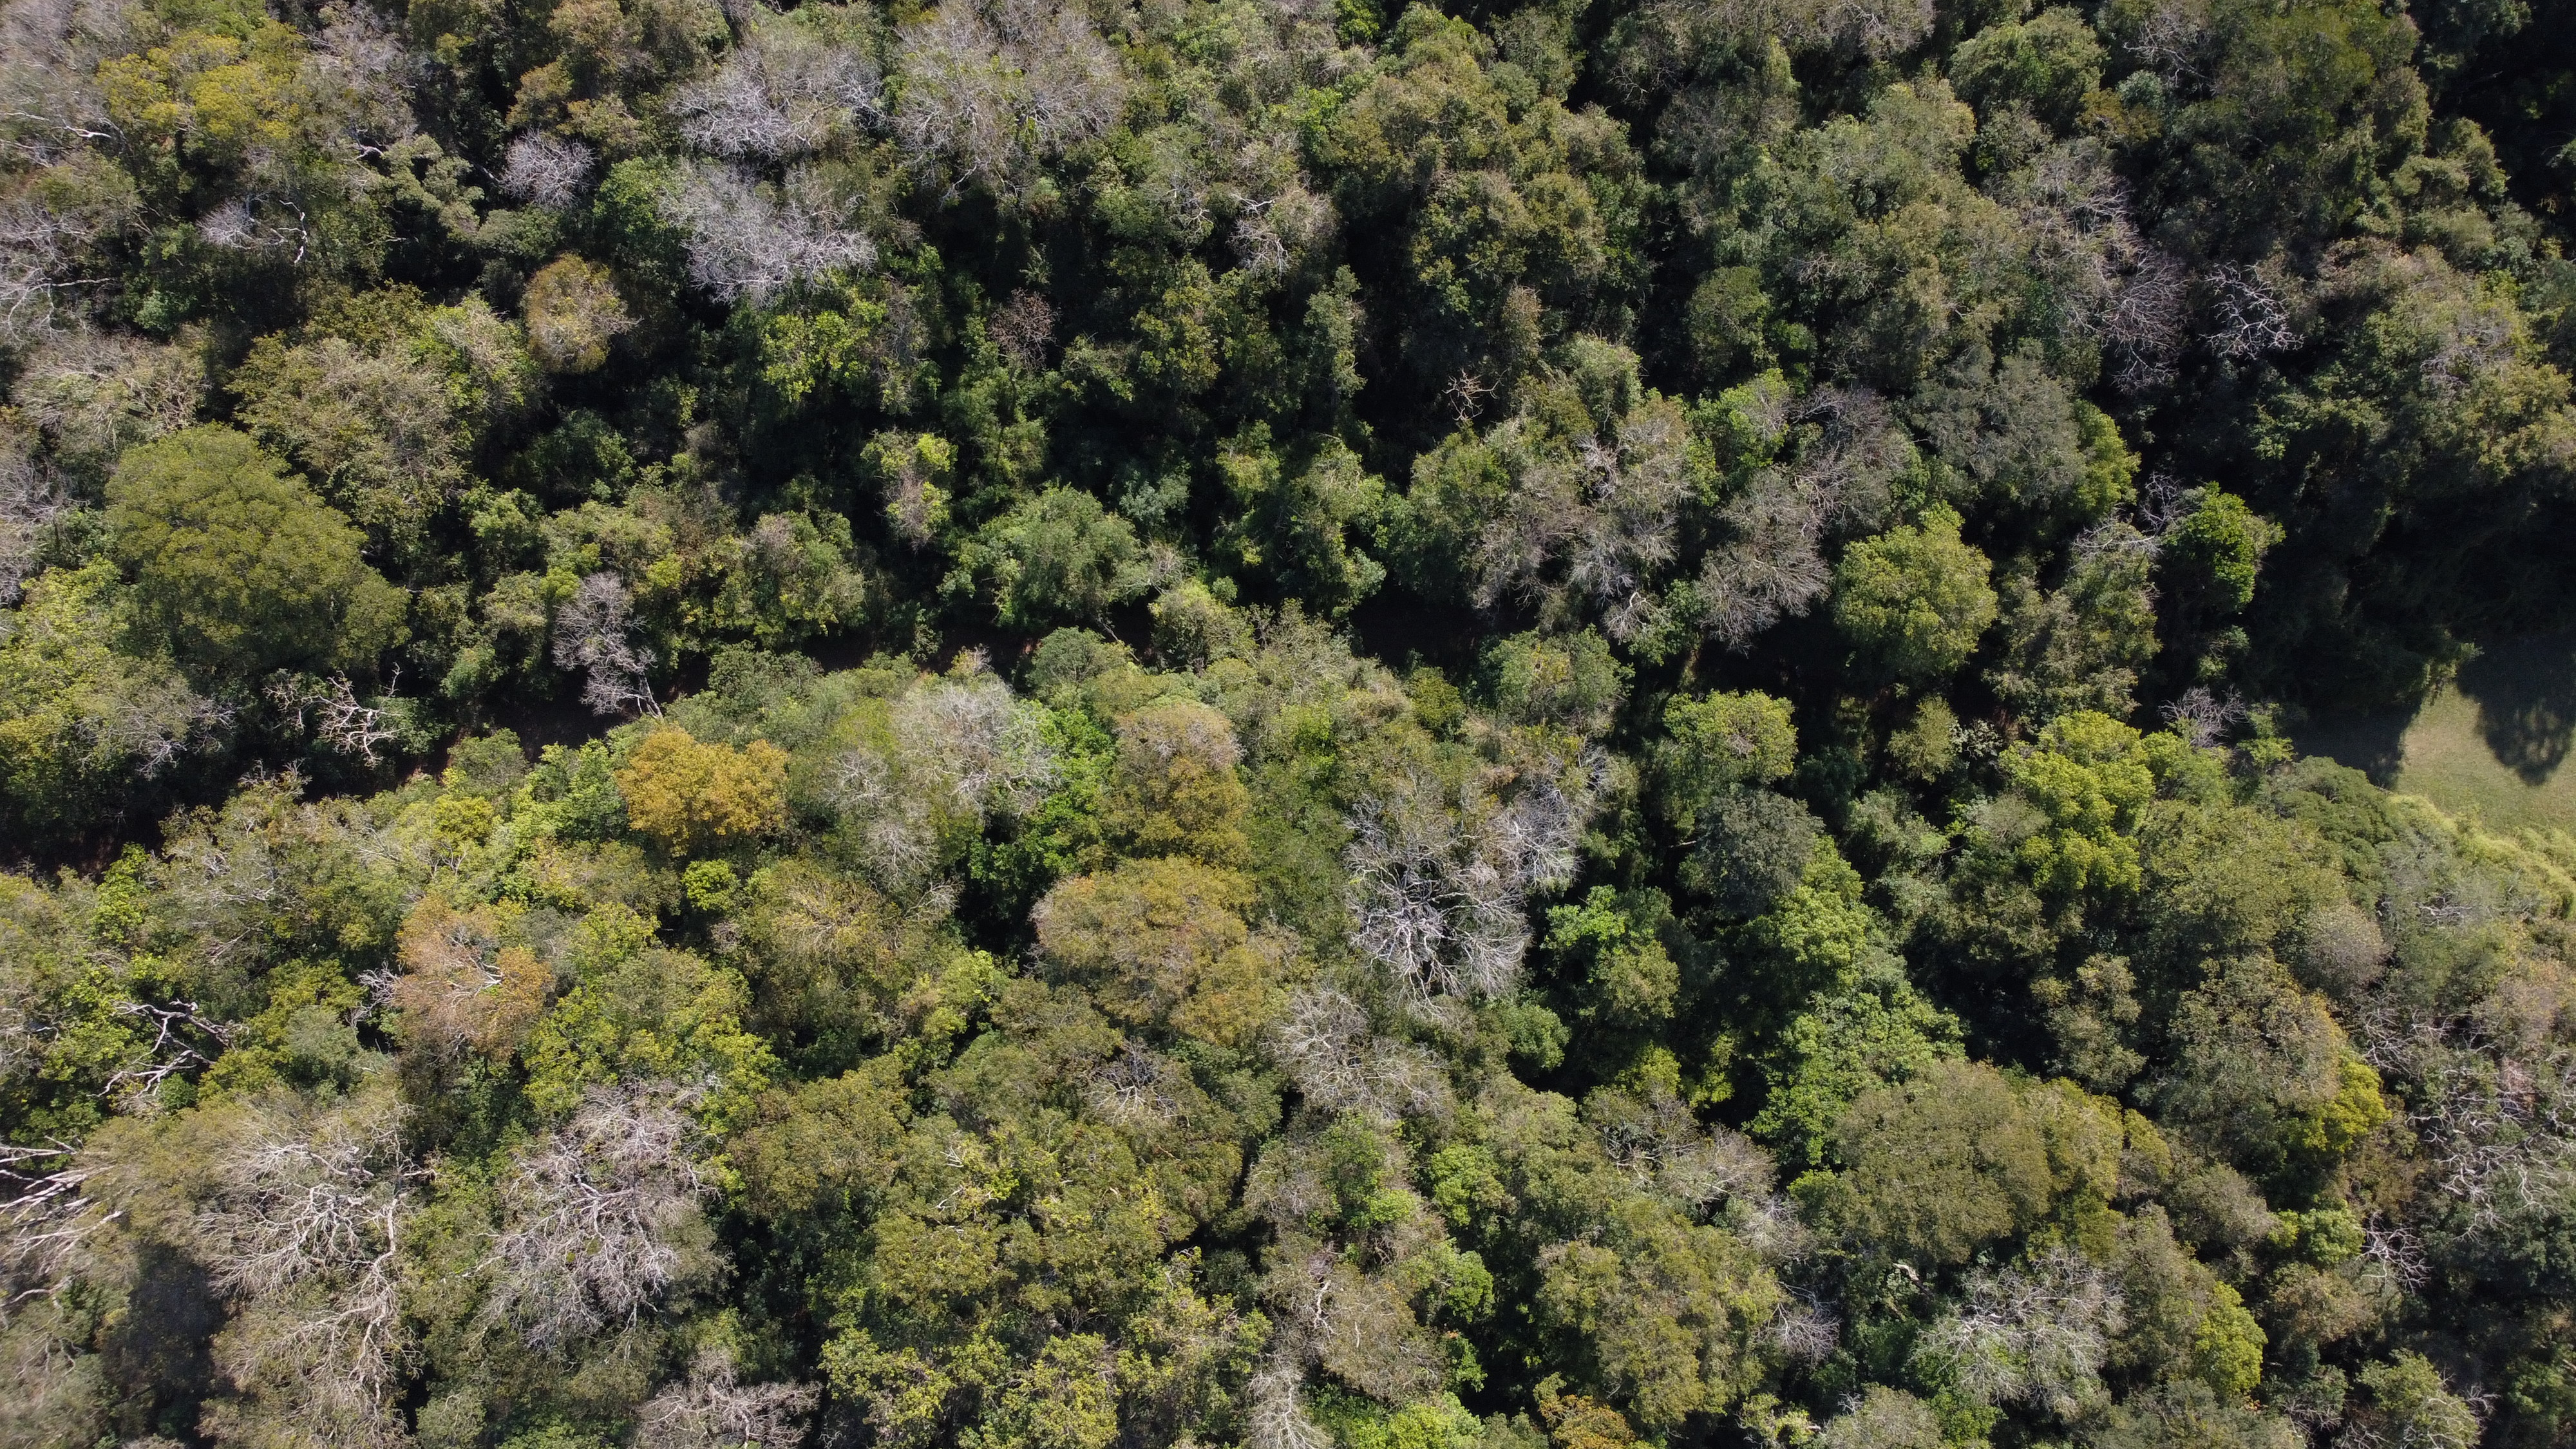
\includegraphics[width=\textwidth]{Imagenes/Homomorfico/DJI_0340.JPG}
     \hfill
     \caption{Imagen aérea (VANT) de reserva provincial Cañadón de Profundidad. Resolución de imagen de N x M píxeles, resolución espacial de X m por píxel.}
    \label{Cañadon_homo2}
\end{figure}

\begin{figure}[h!]
    \includegraphics[width=\textwidth]{Imagenes/Homomorfico/DJI_340_bin.png}
     \hfill
     \caption{Máscara binaria obtenida a partir de la imagen de la figura \ref{Cañadon_homo} con umbral de 0,45.}
    \label{mascaraCañadon2}
\end{figure}

\begin{figure}[h!]
    \includegraphics[width=\textwidth]{Imagenes/Homomorfico/DJI_340_bin.png}
     \hfill
     \caption{Sombras seleccionadas por el algoritmo a partir de la imagen de la figura \ref{mascaraCañadon}.}
    \label{seleccionadaCañadon2}
\end{figure}